
\begin{figure}[t!]
    \centering
    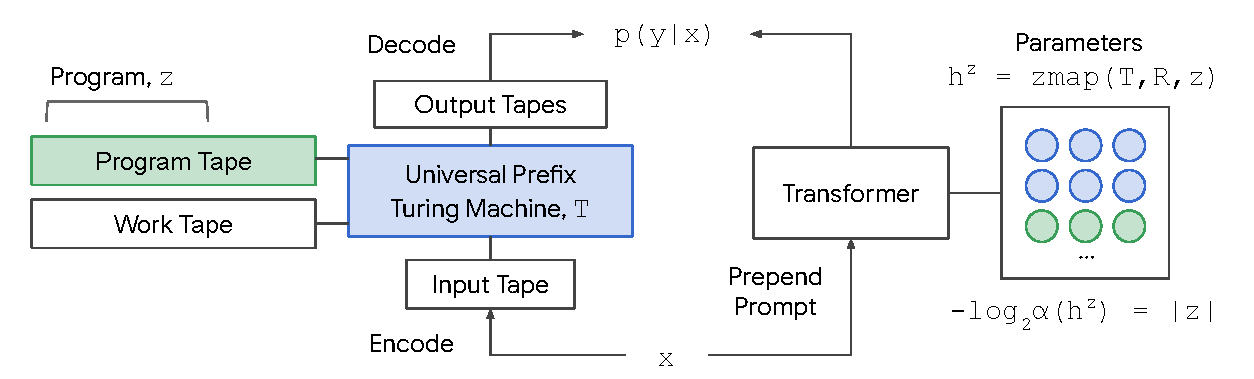
\includegraphics[width=0.75\columnwidth,keepaspectratio]{figures/transformer_turing_emulator_pdf.pdf}
    \caption{\textbf{Constructing asymptotically optimal codes for Transformers.} We construct a function $\zmap$ that establishes that a Transformer (right) can effectively simulate a prefix Turing machine $T$ with any prefix $z$ encoded on a program tape (left), and therefore can represent any computable model function (as defined in section~\ref{sec:problem-setting}) within some arbitrary time and space resource bound $R$. With this mapping between model functions and Transformer parameters established, we can select a prior that assigns probability to sets of parameters based on the algorithmic complexity of the function they compute, thus forming an asymptotically optimal code (Section~\ref{sec:two-part-codes-for-transformers}).}
    \label{fig:transformer_turing_emulator}
\end{figure}
